% !TEX TS-program = xelatex
% !TEX encoding = UTF-8
%
%
\documentclass[a4paper,12pt]{article}
\usepackage[T1]{fontenc}
\usepackage{geometry,anysize,changepage,calc,hyperref,cite,fancyhdr,setspace}
\usepackage{amsmath,amssymb,amsthm,listings,xcolor}
\newtheorem{assumption}{Assumption}

\colorlet{punct}{red!60!black}
\definecolor{background}{HTML}{EEEEEE}
\definecolor{delim}{RGB}{20,105,176}
\colorlet{numb}{magenta!60!black}
\lstdefinelanguage{json}{
    basicstyle=\normalfont\ttfamily,
    numbers=left,
    numberstyle=\scriptsize,
    stepnumber=1,
    numbersep=8pt,
    showstringspaces=false,
    breaklines=true,
    frame=lines,
    backgroundcolor=\color{background},
    literate=
     *{0}{{{\color{numb}0}}}{1}
      {1}{{{\color{numb}1}}}{1}
      {2}{{{\color{numb}2}}}{1}
      {3}{{{\color{numb}3}}}{1}
      {4}{{{\color{numb}4}}}{1}
      {5}{{{\color{numb}5}}}{1}
      {6}{{{\color{numb}6}}}{1}
      {7}{{{\color{numb}7}}}{1}
      {8}{{{\color{numb}8}}}{1}
      {9}{{{\color{numb}9}}}{1}
      {:}{{{\color{punct}{:}}}}{1}
      {,}{{{\color{punct}{,}}}}{1}
      {\{}{{{\color{delim}{\{}}}}{1}
      {\}}{{{\color{delim}{\}}}}}{1}
      {[}{{{\color{delim}{[}}}}{1}
      {]}{{{\color{delim}{]}}}}{1},
}
\renewcommand{\lstlistingname}{Code}
\renewcommand{\lstlistlistingname}{\lstlistingname List}% List of Listings -> List of Algorithms
\definecolor{capri}{rgb}{0.0, 0.75, 1.0}


\usepackage{graphicx,wrapfig,multirow,diagbox,caption,subcaption,enumitem}
\usepackage{verbatim,algpseudocode}
\usepackage[boxruled]{algorithm2e}
\renewcommand{\listalgorithmcfname}{Algorithm List}
\renewcommand{\algorithmcfname}{Algorithm}
\usepackage[numbers,sort,compress]{natbib}
\usepackage{url,bm,titling,mathrsfs}
\newcommand{\lookup}{\text{lookup}}
\newcommand{\net}{\text{net}}
\newcommand{\device}{\text{device}}
\newcommand{\enabstractname}{Abstract}
\newcommand{\cnabstractname}{Abstract}
\newenvironment{enabstract}{
  \par\small
  \noindent\mbox{}\hfill{\bfseries \enabstractname}\hfill\mbox{}\par
  \vskip 2.5ex}{\par\vskip 2.5ex}
\newenvironment{cnabstract}{
  \par\small
  \noindent\mbox{}\hfill{\bfseries \cnabstractname}\hfill\mbox{}\par
  \vskip 2.5ex}{\par\vskip 2.5ex}
% \bibliographystyle{abbrvnat}
% \setcitestyle{open={(},authoryear,close={)}}
\bibliographystyle{unsrtnat}
\listfiles
../doc-EN/initialset.tex
\linespread{1.5}
\newcommand\blfootnote[1]{%
  \begingroup
  \renewcommand\thefootnote{}\footnote{#1}%
  \addtocounter{footnote}{-1}%
  \endgroup
}
% \author{Zichao Long}
\author{Zichao Long, Lin Li, Lei Han, Xianglong Meng, Chongjun Ding,\\
Ruiyan Li, Wu Jiang, Fuchen Ding, Jiaqing Yue, Zhichao Li,\\
Yisheng Hu, Ding Li, $\text{Heng Liao}^\star$}
\setlength{\droptitle}{-10em}
\title{Computational Graph Representation of Equations System Constructors in Hierarchical Circuit Simulation}
\date{}
\begin{document}
\maketitle
\vspace{-5.7em}
\begin{abstract}
  Equations system constructors of hierarchical circuits play a central role in
  device modeling, nonlinear equations solving, and circuit design automation.
  However, existing constructors present limitations in applications to different
  extents. For example, the costs of developing and reusing device models ---
  especially coarse-grained equivalent models of circuit modules ---
  remain high while parameter sensitivity analysis is complex and inefficient.
  % method % avoid introducing background
  Inspired by differentiable programming and
  leveraging the ecosystem benefits of open-source software, we propose
  an equations system constructor using the computational graph representation,
  along with its JSON format netlist, to address these limitations.
  This representation allows for runtime dependencies between signals and
  subcircuit/device parameters. The proposed method streamlines the model
  development process and facilitates end-to-end computation of gradients of
  equations remainders with respect to parameters.
  % overall idea
  This paper discusses in detail the overarching concept of hierarchical
  subcircuit/device decomposition and nested invocation by drawing parallels to
  functions in programming languages, and introduces
  rules for parameters passing and gradient propagation across
  hierarchical circuit modules.
  % examples and conclusions
  The presented numerical examples, including (1) an uncoupled CMOS model
  representation using "equivalent circuit decomposition+dynamic parameters"
  and (2) operational amplifier (OpAmp) auto device sizing, have demonstrated
  that the proposed method supports circuit simulation and design and
  particularly subcircuit modeling with improved efficiency, simplicity,
  and decoupling compared to existing techniques.
  \\
  {\bf{Keywords}}: hierarchical circuit simulation, SPICE, computational graph,
  circuit static parameters, runtime variables, automatic differentiation,
  circuit behavior model, MOS sizing
\blfootnote{$\text{Corresponding author}^\star$}
\end{abstract}

\newpage
\tableofcontents

\newpage
../doc-EN/sec-intro.tex
\section[Hierarchical Circuit Equations System Constructor: Computational Graph]{Hierarchical Circuit Equations System Constructor: \\ Computational Graph}\label{sec:Joanna}
\begin{figure}[htpb]
  \centering
  \begin{subfigure}{0.49\textwidth}
    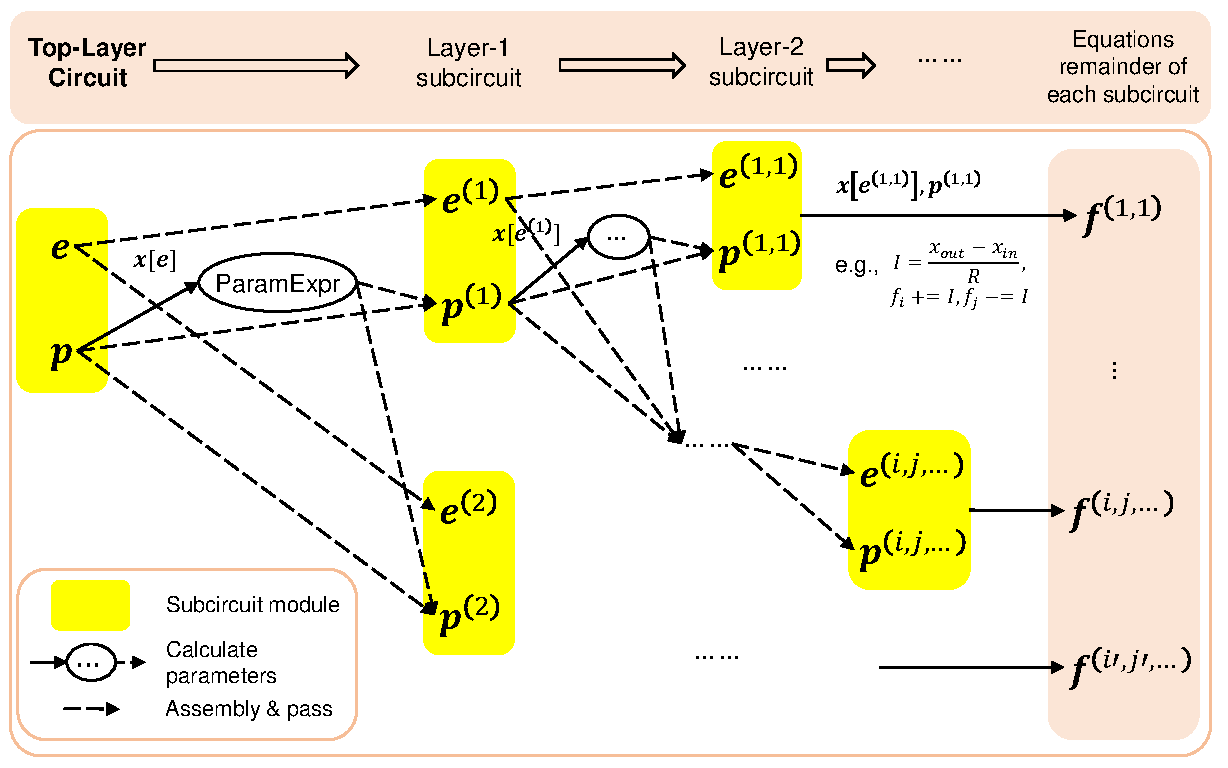
\includegraphics[width=\textwidth]{fig/static-engine.pdf}
    \caption{现有技术:静态参数}
    \label{fig:static-engine}
  \end{subfigure}
  \begin{subfigure}{0.49\textwidth}
    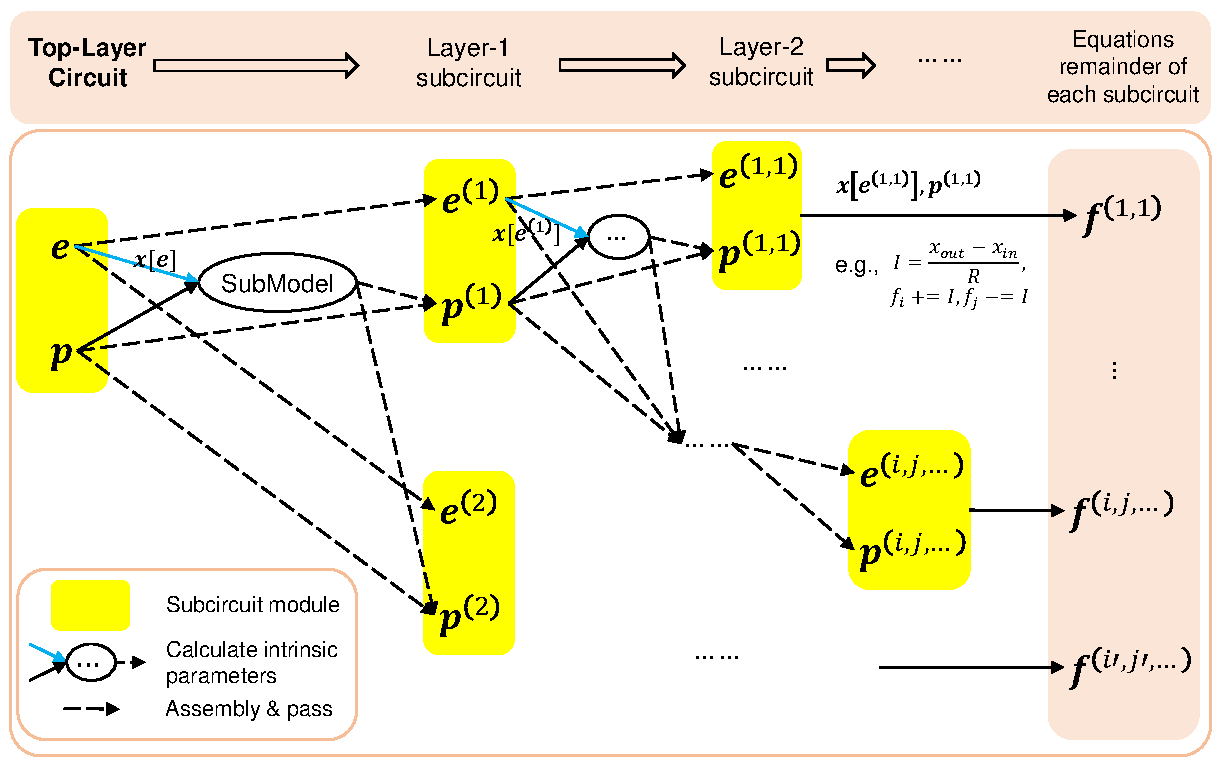
\includegraphics[width=\textwidth]{fig/computational-graph.pdf}
    \caption{计算图:动态参数}
    \label{fig:computational-graph}
  \end{subfigure}
  \caption{层次电路方程组构建器:
  现有技术\ref{fig:static-engine} v.s. 计算图\ref{fig:computational-graph}。
  每个计算单元({\color{yellow}黄色模块})对应一个子电路,
  可逐层分解为更小的子电路,其中最小粒度子电路为“基本器件”。
  $\bm{e}^{(\cdots)}$ 表示对应子电路的内外节点,$\bm{x}$ 是广义信号,
  如节点偏置电压、支路电流;
  $\bm{p}^{(\cdots)}$ 表示该子电路涉及的输入参数,如器件尺寸,
  对于动态参数而言还可以是基本器件的非线性电容、电感、电流值等;
  $\bm{f}^{(\cdots)}$ 是子电路对仿真方程余项的贡献,
  示意图中省略了 Jacobian 矩阵的计算。
  现有技术中,电路模块下层参数不依赖于信号值$\bm{x}[\bm{e}]$,
  可在网表编译期完成 ParamExpr 的计算;
  计算图中,动态参数来自 SubModel 输出的{\color{capri}内部变量},
  在方程组计算的运行时获得。
  }
  \label{fig:equations-system-constructor}
\end{figure}
% \subsection{符号 \& 背景}
给定 $N$ 个广义信号(即方程未知数) $\bm{x}\in\mr^N$
及 $M$ 个与信号无关的输入变量或参数 $\bm{p}\in\mr^M$,
数学上,电路仿真本质是“构建+求解”如下守恒型代数微分方程
\cite{najm2010circuit,gunther2005modelling,hu2020adjoint}
\begin{equation}\label{eq:flat-equation}
  \bm{f}(\bm{\dot{x}}(t),\bm{x}(t),\bm{p})
  \triangleq\frac{\ud\bm{Q}(\bm{x},\bm{p})}{\ud t}+\bm{F}(\bm{x},\bm{p})
  =\bm{0},\tag{Eq.(Flat)}
\end{equation}
其中,$\bm{Q}$ 是方程余项的动态部分,例如电容器的电荷、电感器的磁通量;
$\bm{F}$ 是方程余项的静态部分,如节点总流入直流电流,电压源压降方程。
% Hierarchical 仿真: Cadence UltraSim, Synopsys HSPICE;
现代仿真器通常将 \ref{eq:flat-equation} 按照电路层次进行分解和构建,
具有更易理解、并行的优点:
\begin{equation}\label{eq:hierarchical-equation}
  \begin{split}
    \bm{f}(\bm{\dot{x}},\bm{x},\bm{p})
    & = \bm{f}^{(1)}(\bm{\dot{x}}^{(1)},\bm{x}^{(1)},\bm{p}^{(1)})
    + \bm{f}^{(2)}(\bm{\dot{x}}^{(2)},\bm{x}^{(2)},\bm{p}^{(2)})
    + \cdots \\
    & = \bm{f}^{(1,1)}+\bm{f}^{(1,2)}+\cdots+\bm{f}^{(2,1)}+\bm{f}^{(2,2)}+\cdots, \\
    & \cdots
  \end{split}\tag{Eq.(Hierarchical)}
\end{equation}
其中 $\bm{x}^{(i)},\bm{p}^{(i)},\bm{f}^{(i)}$ 分别是原电路的
第 $i$ 个子电路的输入信号、参数或变量及贡献的方程余项,
$\bm{x}^{(i)},\bm{f}^{(i)}$ 之间相互交叠的部分取决于各子电路公共节点。
如 \ref{eq:hierarchical-equation} 所示,$\bm{f}^{(i)}$ 也可按需进一步
逐级分解为 $\bm{f}^{(i,1)},\bm{f}^{(i,2)},\cdots$ 等。

需要说明的是,\ref{eq:flat-equation} 仅表示瞬态(TRAN)分析方程,数值求解时
常常将 \ref{eq:flat-equation} 沿时间方向离散,并在每个时间步使用如 Newton-Raphson
方法求解代数方程组
\cite[Sec 7.1]{fijnvandraat2002time}
\[
  \text{ Solve }\bm{x},\text{ Subject to }
  \frac{1}{\beta\Delta t}\bm{Q}(\bm{x},\bm{p})+F(\bm{x},\bm{p})+\bm{b}=\bm{0},
\]
需反复计算 $\bm{Q},\bm{F}$ 及稀疏 Jacobian 矩阵
$\nabla_{\bm{x}}\bm{Q},\nabla_{\bm{x}}\bm{F}$。 若考虑其他如直流(DC)分析,
交流(AC)小信号分析,则需对 \ref{eq:flat-equation} 进行转换
(附录\ref{appendix:TRAN-to-AC-equation})。 由于各分析对应方程的处理是类似的,
下面主要以TRAN分析和一个简单的 JSON 网表子电路定义
(代码块\ref{lst:size-dependent-resistor})
为例,着重说明在层次电路仿真中,如何将
$\bm{Q}^{(\cdots)},\bm{F}^{(\cdots)}$,
$\nabla_{\bm{x}^{(\cdots)}\text{ or }\bm{p}^{(\cdots)}}\bm{Q}^{(\cdots)}$,
$\nabla_{\bm{x}^{(\cdots)}\text{ or }\bm{p}^{(\cdots)}}\bm{F}^{(\cdots)}$
的计算过程表达为计算图(图\ref{fig:computational-graph})的前传和反传。


\subsection{JSON网表中的子电路模块定义}
\label{subsec:subckt-module-definition}
类似于 Verilog-A/MS\cite[Sec 6]{verilog2014verilog},
定义一个电路模块,应该包含五部分信息(表\ref{tab:subckt-module-definition}):
(1)外部节点;(2)内部节点;(3)输入参数;(4)内部子电路分解;(5)内部变量。
\begin{lstlisting}[language=json,basicstyle=\small,numbers=none,
caption={网表中自定义名为 “SizeDepResistor” 的子电路:由尺寸决定阻值的电阻器},
label=lst:size-dependent-resistor]
"SizeDepResistor":{ # 定义子电路模块
  “ExternalNodes":["l","r"],
  “InputParams":["Rlength","Rwidth"],
  “InternalNodes":[],
  “SubModel":{
    “Expr":"[1e2*Rlength/Rwidth,]",
    “IntrinsicParams":["RValue"]
  },
  “Schematic":{ # 模块内各子电路/器件实例化语句
    “instanceR":{
      “MasterName":"resistor",
      “ExternalNodes":{"left":"l","right":"r"},
      “InputParams":{"resistance":"RValue"}
    }
  }
}
\end{lstlisting}
\begin{table}[htbp]
  \centering
  \caption{子电路模块定义}\label{tab:subckt-module-definition}
  \begin{tabular}{l|l|l|l}
    \hline
    & \multicolumn{1}{c|}{内容} & \multicolumn{1}{c|}{字段} & \\
    \hline
    \multirow{4}{*}{\begin{tabular}[c]{@{}r@{}}结构信息\\{\small(字典+列表)}\end{tabular}}
    & 外接节点名列表 & ExternalNodes & 必须 \\
    & 内部节点名列表 & InternalNodes & 必须 \\
    & 输入参数名列表 & InputParams   & 必须 \\
    & 内部子电路分解 & Schematic     & 必须 \\
    \hline
    \begin{tabular}[c]{@{}r@{}}行为信息\\{\small(可微函数映射)}\end{tabular}
    & 内部变量子模型 & SubModel      & 可选 \\
    \hline
\end{tabular}
\end{table}
其中,“Schematic”字段表示内部子电路分解,其中包含零或若干个子电路/器件的实例化语句,
每个实例化语句的组成是 (1)实例名;(2)类型名;(3)对外节点连接;(4)输入参数值。
以代码块\ref{lst:size-dependent-resistor}为例,其子电路分解中仅包含一个实例,
\begin{itemize}[partopsep=0pt,topsep=0pt,itemsep=0pt,parsep=0pt]
  \item “instanceR” 是实例名称。
  \item “MasterName” 指出该实例的类型是 “resistor”。
    实例类型可以是其他子电路模块,也可以是内部支持的基本器件类型。
  \item “ExternalNodes” 指出该实例的两个外接节点 “left”,“right” 连接在
    当前模块,即 “SizeDepResistor” 的 “l”,“r” 上。
    一般情况下,“Schematic” 中各个实例所连接的节点应当
    来自于当前模块的内外节点:“ExternalNodes” 以及 “InternalNodes”。
  \item “InputParams” 指出该实例的参数是 “SubModel” 子模型计算出来的内部变量
    “RValue”。一般情况下,“Schematic” 中实例所引用的参数来自于:
    (1)全局变量;
    (2)当前模块的“InputParams”;
    (3)当前模块 “SubModel” (如果有)下的 “IntrinsicParams”。
\end{itemize}
关于 SubModel 及其作用的更多讨论参考下文 Sec \ref{subsec:EvalCompositeSubCkt}。

\subsection{子电路模块实例在程序中的表示}
\label{subsec:subckt-instance-data-structure}
% 无需 EvalCompositeSubCkt 算法细节,梳理数据
为使方程组构建器可高效调用子电路模块,子电路定义
应当编译为合适的层次化数据结构(图\ref{fig:subckt-instance-data-structure}),
每个子电路模块定义经编译后通常包含两部分:
(1)同类子电路共享规则(表\ref{tab:BasicCompositeSubCktRule});
(2)实例私有数据(表\ref{tab:CompositeSubCkt})。
\begin{figure}[htpb]
  \centering
  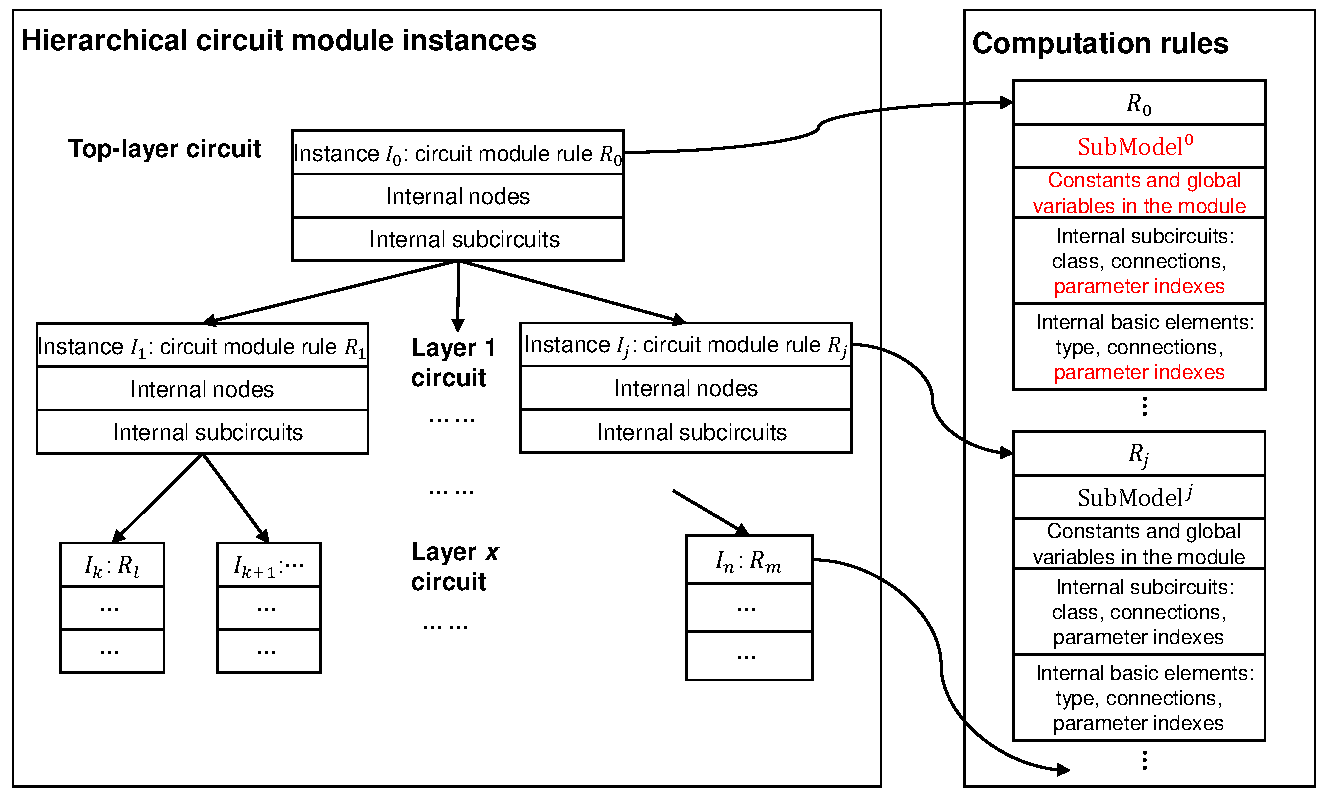
\includegraphics[width=0.8\textwidth]{fig/subckt-instance-data-structure.pdf}
  \caption{层次子电路模块实例及计算规则示意。
  {\color{red}红色字体}部分是与现有技术\cite{tcherniaev2003transistor}的不同点:
  现有技术不需要支持动态参数,因此仅需在各电路模块计算规则中存储器件的固定参数;
  本方法中传递给下层实例、器件的参数均在运行时计算,因此需建立参数的索引。}
  \label{fig:subckt-instance-data-structure}
\end{figure}
\begin{table}[htbp]
  \centering
  \caption{子电路模块实例数据}\label{tab:CompositeSubCkt}
  \begin{tabular}{l|l}
    \hline
    \multicolumn{1}{c|}{符号} & \multicolumn{1}{c}{含义} \\
    \hline
    rule        & 指向该类子电路规则(表\ref{tab:BasicCompositeSubCktRule})的指针 \\
    \textbf{in} & 子电路实例的内部节点序号,\textbf{i}nternal \textbf{n}odes \\
    subckts     & 下层子电路实例指针 \\
    \hline
  \end{tabular}
\end{table}
\begin{table}[htbp]
  \centering
  \caption{子电路模块计算规则}\label{tab:BasicCompositeSubCktRule}
  \begin{tabular}{l|l}
    \hline
    \multicolumn{1}{c|}{符号} & \multicolumn{1}{c}{含义} \\
    \hline
    \textbf{c}       & 常数参数                                    \\
    \textbf{gv}      & 全局变量                                    \\
    SubModel         & 用于计算内部变量的子模型 \\
    SubCktsInfo      & 下层子电路节点、参数索引 \\
    BasicElementInfo & 基本器件节点、参数索引 \\
    \hline
  \end{tabular}
\end{table}
有几点需要说明
\begin{enumerate}[partopsep=0pt,topsep=0pt,itemsep=0pt,parsep=0pt]
  \item 各层子电路的外接节点来自上层子电路。
    其中,顶层电路应构成封闭系统,无外接节点。
  \item 不同子电路实例可能共用外部节点,但独享内部节点。
    实例化子电路时需注意使各内部节点互不冲突。
  \item 全局变量与系统信号 $\bm{x}$ 对于所有子电路模块均全局可见,
    模块计算规则(表\ref{tab:BasicCompositeSubCktRule})中仅需存储对所有全局变量
    的索引 \textbf{gv},模块内外节点也均以序号即索引形式存储及传递。
  \item 如果需要更多用于支持交互式分析及 Debug 的信息:
    可在计算规则(表\ref{tab:BasicCompositeSubCktRule})
    中添加子电路类型名、内外节点参数名、下层子电路实例化语句,
    甚至在实例(表\ref{tab:CompositeSubCkt})中动态记录输入变量
    (\textbf{i}nput \textbf{p}arameters) \textbf{ip} 等。
\end{enumerate}

\subsection{子电路模块定义到实例的编译}
\label{subsec:subckt-module-compilation}
JSON 网表文件的解析可借助程序语言的 JSON 解析工具,而子电路模块定义
(Sec \ref{subsec:subckt-module-definition})的编译分为两个步骤
\begin{enumerate}[partopsep=0pt,topsep=0pt,itemsep=0pt,parsep=0pt]
  \item 编译所有子电路模块的计算规则(图\ref{fig:compile-subckt-rule})。
    这里 SubModel 的解析与编译取决于编译器本身的实现,
    其他结构信息的处理,即节点、参数索引的建立,只需使用最基本的
    算法和数据结构如列表、字典即可完成。
  \item 递归实例化层次电路模块(图\ref{fig:cktrule-to-subckt})。
    其中,从顶层电路启动实例化程序时,输入的节点序号偏置$n=0$。
    图中所示方法保证了各个子电路模块的内部节点是相互独立的。
\end{enumerate}
\begin{figure}[htpb]
  \centering
  \begin{subfigure}{0.59\textwidth}
    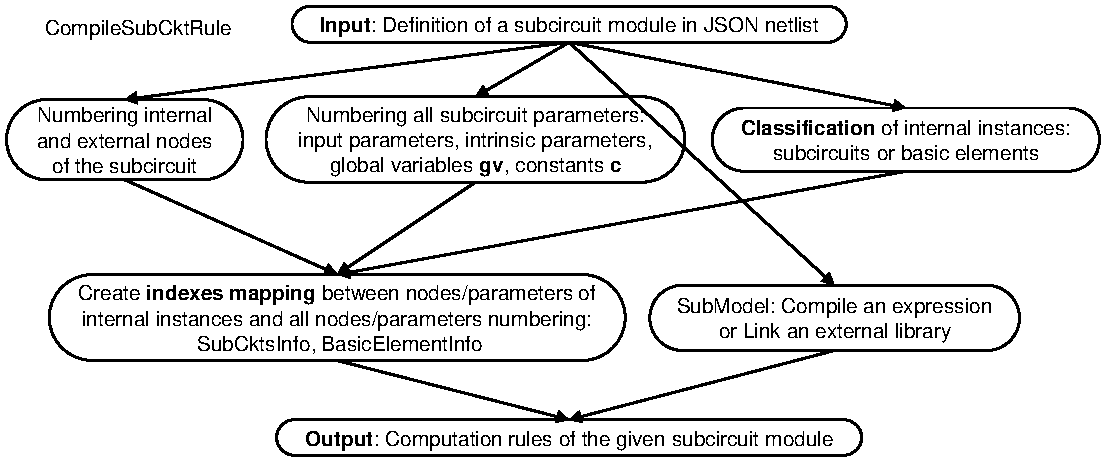
\includegraphics[width = \textwidth]{fig/compile-subckt-rule.pdf}
    \caption{编译单个模块的计算规则}
    \label{fig:compile-subckt-rule}
  \end{subfigure}
  \begin{subfigure}{0.35\textwidth}
    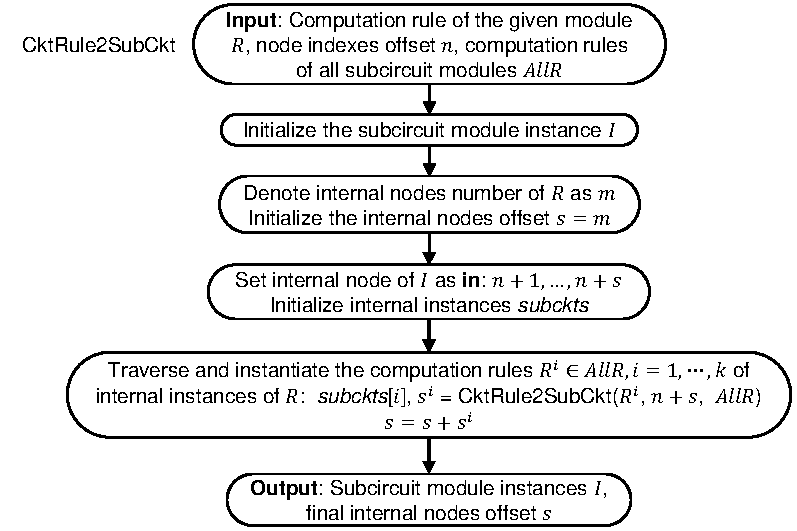
\includegraphics[width = \textwidth]{fig/cktrule-to-subckt.pdf}
    \caption{递归实例化}
    \label{fig:cktrule-to-subckt}
  \end{subfigure}
  \caption{电路模块编译}
  \label{fig:subckt-module-compilation}
\end{figure}
需要注意的是,电路模块内部子电路分解可同时包含下层电路模块和基本器件,
因此编译器也需识别哪些实例是基本器件,哪些实例是网表中定义的子电路模块,
并分别建立节点、参数的索引。
其他内容,如检查子电路类型是否有循环定义、网表是否包含未定义子电路模块、
电路连通性、电路中是否有未用到的节点等检查,这里不再赘述。
\paragraph{基本器件}
\addcontentsline{toc}{subsubsection}{\ \ \ \ 基本器件}
可以认为是内置支持的最小粒度子电路,没有内部节点、内部器件,
当前支持的基本器件部分列表可参考表\ref{tab:basic-elements-partial-list}。
若要新增一种基本器件,需完成的工作包括(1)定义各分析下的电学响应函数;
(2)为编译器提供外接节点、输入参数等信息。
\begin{table}[htpb]
  \centering
  \caption{部分基本器件列表}
  \label{tab:basic-elements-partial-list}
  \begin{tabular}{l|l|l|l}
    \hline
     \multicolumn{1}{c}{MasterName}   & \multicolumn{1}{|c|}{ExternalNodes} &
     \multicolumn{1}{c|}{InputParams} & 备注             \\
    \hline
     resistor   & left,right              & resistance  & 电阻器           \\
     capacitor  & input,output            & capacitance & 电容器           \\
     inductor   & input,output            & inductance  & 电感器           \\
     CS         & input,output            & current     & 电流源           \\
     VS         & input,output            & voltage     & 电压源           \\
     VCCS       & left,right,input,output & MF          & 电压受控电流源   \\
     CCCS       & iorigin,input,output    & MF          & 电流受控电流源   \\
     VCVS       & left,right,input,output & MF          & 电压受控电压源   \\
     CCVS       & iorigin,input,output    & MF          & 电流受控电压源   \\
    \hline
  \end{tabular}
\end{table}

值得说明的是,按照改进的节点分析法\cite{ho1975modified},
电压源类型的基本器件必须将支路电流也作为一个自由度,
在编译器中处理为该器件外接 GALV 节点,相应的,
编译时需在上层模块新增一个内部节点。
非电压源类基本器件如电阻器也可增加一个广义外接 GALV 节点,
该节点信号通常表示流经器件支路的电流,以 TRAN 分析为例,
记电阻器的阻值为 $R$,左右节点是 $l,r$,电压值 $x_l,x_r$,
GALV 节点(如果有)及电流值是 $i,x_i$,则电阻器对应的方程余项以稀疏向量表示是
\begin{description}
  \item[无外接 GALV:] $\bm{Q}=\bm{0},\bm{F}=[(l,-\frac{x_l-x_r}{R}),(r,\frac{x_l-x_r}{R})]$。
  \item[外接 GALV:] $\bm{Q}=\bm{0},\bm{F}=[(l,-x_i),(r,x_i),(i,x_r-x_l+R\cdot x_i)]$。
\end{description}
这实际上就是\cite[Sec 2.4.4]{najm2010circuit}中同类器件的
不同 element stamp,也可理解为同类器件的
两种网络分析方法\cite{ho1975modified,hachtel1971sparse},
这一特性需要编译器与方程组构建器同时支持。
在不同仿真分析中,基本器件仿真方程余项和梯度的计算需加以区分,这里不再详细讨论。

\subsection{执行:计算图的前传和反传}\label{subsec:EvalCompositeSubCkt}
计算图\ref{fig:computational-graph}的每个基本计算单元对应一个子电路实例。
当子电路在计算图中被调用时,计算单元
首先从上层电路输入外接节点、输入变量,然后遍历内部子电路、基本器件以计算
方程余项、信号梯度、变量梯度,最后将这些结果返回给上层。
计算单元的内部过程可表达为算法\ref{alg:EvalCompositeSubCkt}:\\
\begin{algorithm}[H]
  % \TitleOfAlgo{调用子电路}
  \caption{调用子电路\\
  方程余项,信号梯度,变量梯度 = EvalCompositeSubCkt($\bm{x}$, ckt, \textbf{en}, \textbf{ip})}
  \label{alg:EvalCompositeSubCkt}
  \SetAlgoLined
  输入:所有系统信号 $\bm{x}$,子电路实例 ckt,外接节点下标 \textbf{en},输入变量 \textbf{ip}\;
  \# ckt 内部可获得信息:内部节点 \textbf{in},子模型 SubModel,全局变量 \textbf{gv},常数 \textbf{c}\;
  1. 组装 ckt 内部节点 \textbf{in} 和外接节点 \textbf{en} 得到 \textbf{nodes}=[\textbf{en},\textbf{in}]\;
  2. 依据内外信号及输入变量计算内部变量 \textbf{intrp} = 
  SubModel($\bm{x}$[\textbf{nodes}],\textbf{ip})\;
  3. 组装 ckt 当前所有变量及参数得到 \textbf{params}=
  [\textbf{ip},\textbf{intrp},\textbf{gv},\textbf{c}]\;
  4. 从 \textbf{nodes},\textbf{params} 提取 ckt 内部各子电路 subckt
  外接节点 \textbf{suben}$\subset$\textbf{nodes}、
  输入变量 \textbf{subip}$\subset$\textbf{params},
  并调用 EvalCompositeSubCkt($\bm{x}$, subckt, \textbf{suben}, \textbf{subip})\;
  % $\bm{Q},\bm{F},\nabla_{\bm{x}}\bm{Q},\nabla_{\bm{x}}\bm{F}$,$\nabla_{\bm{gv}}\bm{Q},
  % \nabla_{\bm{subip}}\bm{Q},\nabla_{\bm{gv}}\bm{F},\nabla_{\bm{subip}}\bm{F}$\;
  5. 从 \textbf{nodes},\textbf{params} 提取 ckt 内部各基本器件外接节点、输入变量并
  计算各基本器件的方程余项、梯度\;
  6. 收集4,5步的所有方程余项\;
  7. 依据 1-5 下标映射,反传下层子电路、基本器件的信号梯度及变量梯度\;
  输出:方程余项,信号梯度,变量梯度
\end{algorithm}
\vspace{\parsep}
\begin{figure}[htpb]
  \centering
  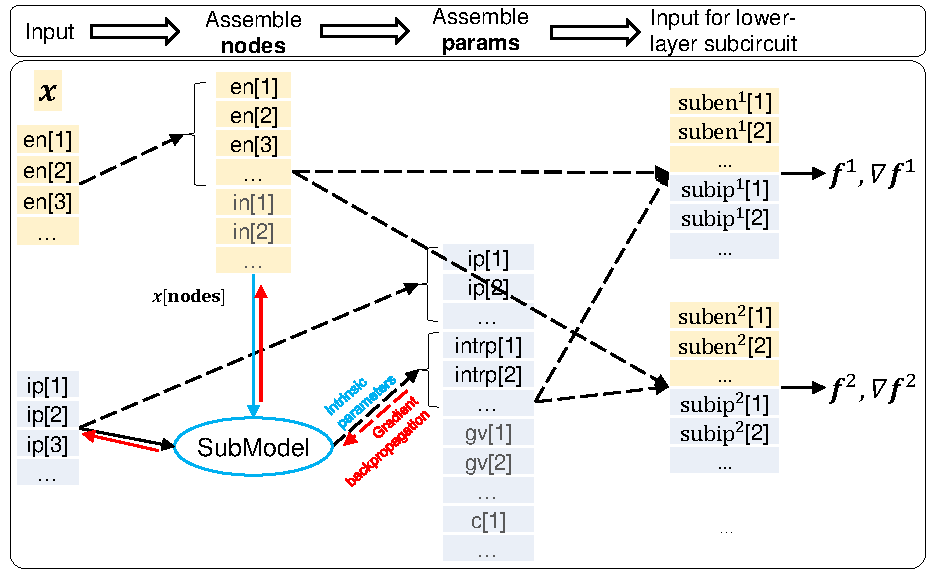
\includegraphics[width=0.7\textwidth]{fig/EvalCompositeSubCkt.pdf}
  \caption{算法\ref{alg:EvalCompositeSubCkt} 1-5步示意图。
  图\ref{fig:computational-graph}中顶层至第一层子电路调用的放大版。
  现有技术的电路模块中,输入参数和内部参数都可以在编译器计算,
  运行时不反传参数的梯度。}
  \label{fig:EvalCompositeSubCkt}
\end{figure}
这里 \textbf{en},\textbf{ip},\textbf{in},\textbf{gv},\textbf{intrp} 分别是
external nodes, input parameters, internal nodes, global variables,
intrinsic parameters 的缩写。 电路的内外节点\textbf{en},\textbf{in}
可分别用于索引广义信号值 $\bm{x}[\textbf{en}],\bm{x}[\textbf{in}]$。
电路模块涉及的变量/参数 $\bm{p}$ 则由
\textbf{ip},\textbf{gv},\textbf{intrp},\textbf{c} 四部分所组成。
图\ref{fig:EvalCompositeSubCkt}是此算法1-5步的示意图。

\paragraph{SubModel 与内部变量}
\addcontentsline{toc}{subsubsection}{\ \ \ \ SubModel与内部变量}
计算图中,SubModel 起到的作用是,输入当前模块的内外信号及输入变量,
输出所有\textbf{内部变量} \textbf{intrp}=SubModel(\textbf{signals},\textbf{ip})
(其中 \textbf{nodes}=[\textbf{en},\textbf{in}],
\textbf{signals}=$\bm{x}[\textbf{nodes}]$),
这些内部变量可被传递给下层子电路及基本器件。
该设定对应于这样的假设\ref{assumption:intrinsic-params-dependencies}:
“电路模块的行为应由内外信号及输入变量唯一确定”,
因此对 SubModel 而言,
不需要感知下层子电路的内部信号,或其他无关模块的节点信号或参数。
这一设定可以涵盖相当范围的非线性效应,且易于编程实现。
\begin{assumption}\label{assumption:intrinsic-params-dependencies}
  子电路模块中的所有内部变量由子电路内外节点偏置信号和输入变量决定。
\end{assumption}
电路定义中 SubModel 需提供足够信息,使得编译器可将 SubModel 注册到
共享规则(表\ref{tab:BasicCompositeSubCktRule})中,
且计算图和 SubModel 之间应当有某种协议用于获取\textbf{intrp}关于
\textbf{signals},\textbf{ip}的 Jacobian 矩阵:
\vspace{-0.5em}
\begin{equation}\label{eq:submodel-jacobian}
  J_{\textbf{s}} = \nabla_{\textbf{signals}}\textbf{intrp},
  J_{\textbf{ip}}=\nabla_{\textbf{ip}}\textbf{intrp},
\vspace{-0.5em}
\end{equation}
具体实现方式取决于所用的程序语言,这里不再赘述。

\paragraph{逐层梯度反传}
\addcontentsline{toc}{subsubsection}{\ \ \ \ 逐层梯度反传}
计算图调用子电路的计算过程与通常的层次电路方程组计算的主要区别
(图\ref{fig:equations-system-constructor})是:计算图中,
由于下层模块或器件的输入参数 \textbf{subip} 是全部参数 \textbf{params} 的子集
(图\ref{fig:EvalCompositeSubCkt}),因此,还需处理输入变量的梯度的反传。
这里以 TRAN 仿真为例,着重说明在算法\ref{alg:EvalCompositeSubCkt}中如何反传梯度。

对 TRAN 分析而言,算法\ref{alg:EvalCompositeSubCkt}的返回值实际包含8项:
$\bm{Q},\bm{F},\nabla_{\bm{x}}\bm{Q},\nabla_{\bm{x}}\bm{F}$,
$\nabla_{\textbf{gv}}\bm{Q},\nabla_{\textbf{ip}}\bm{Q}$,
$\nabla_{\textbf{gv}}\bm{F},\nabla_{\textbf{ip}}\bm{F}$。
由于 $\bm{Q}$ 与 $\bm{F}$ 的梯度反传没有区别,因此,下面为了简便,仅考虑 $\bm{Q}$。
算法\ref{alg:EvalCompositeSubCkt}中收集到的所有子电路计算结果记做
$\{\bm{Q}^{i}\}$,$\{\nabla_{\bm{x}}\bm{Q}^{i}\}$,
$\{\nabla_{\textbf{gv}}\bm{Q}^{i}\}$,$\{\nabla_{\textbf{subip}^i}\bm{Q}^{i}\}$,
这里上标 $i$ 表示内部子电路或基本器件的序号。
$\bm{Q}^{i}$,$\nabla_{\bm{x}}\bm{Q}^{i}$,$\nabla_{\textbf{gv}}\bm{Q}^{i}$
本身可直接组装,
\[
  \bm{Q} = \sum_i \bm{Q}^{i},
  \nabla_{\bm{x}}\bm{Q} = \sum_i \nabla_{\bm{x}}\bm{Q}^{i},
  \nabla_{\textbf{gv}}\bm{Q} = \sum_i \nabla_{\textbf{gv}}\bm{Q}^{i},
\]
而 $\nabla_{\textbf{subip}^i}\bm{Q}^{i}$ 的梯度反传则需按照 $\textbf{subip}^i$
对\textbf{params}=[\textbf{ip},\textbf{intrp},\textbf{gv},\textbf{c}]
的索引来分情况处理:
\begin{enumerate}[partopsep=0pt,itemsep=0pt,parsep=0pt]
  \item 若 $\text{subip}^i[j]\in\textbf{c}$,则无需反传。
  \item 若 $\text{subip}^i[j]\in\textbf{ip}\cup\textbf{gv}$,
    则直接反传 $\nabla_{\text{subip}^i[j]}\bm{Q}^i$
    至对应的 $\nabla_\textbf{ip}\bm{Q}$ 或 $\nabla_\textbf{gv}\bm{Q}$。
  \item 若有某个下标 $l$,使得 $\text{subip}^i[j]=\textbf{intrp}[l]$
    (图\ref{fig:EvalCompositeSubCkt})。
    注意到前面提到的假设\ref{assumption:intrinsic-params-dependencies}
    及内部变量关于信号与输入变量的 Jacobian 矩阵(式\ref{eq:submodel-jacobian}),
    令 $\bm{g}\triangleq\nabla_{\textbf{subip}^i[j]}\bm{Q}^{i}$,可得
    \vspace{-1em}
    \begin{equation}\label{eq:intrinsic-params-backward}
      \nabla_{x[\textbf{nodes}]}\bm{Q}\mathrel{+}=J_{\textbf{s}}[:,l]\otimes\bm{g},
      \nabla_{\textbf{ip}}\bm{Q}\mathrel{+}=J_{\textbf{ip}}[:,l]\otimes\bm{g}.
    \vspace{-1em}
    \end{equation}
    其中 $\otimes$ 表示两个向量的外积。
\end{enumerate}





\section{Applications}\label{sec:applications}
\subsection{CMOS Device Model: Equivalent Circuit Decomposition + Dynamic Parameters}\label{subsec:cmos-model}
As mentioned earlier, any subcircuit module (e.g., CMOS) that satisfies Assumption \ref{assumption:intrinsic-params-dependencies} can be modeled as a submodel-based representation featuring "equivalent circuit decomposition + dynamic parameters". This section provides an implementation example based on a lookup table. Reimplementing BSIM model \cite{chauhan2012bsim} as a SubModel is a conventional method that offers better compatibility with the existing method, but it is not adopted in this work. The CMOS module definition consists of the following elements (details about the definition are provided in Appendix \hyperref[appendix:mos-subckt]{B} and the equivalent circuit diagram under AC analysis is given in Figure \ref{fig:mos-small-signal-model-2}):
\begin{enumerate}[partopsep=0pt,topsep=0pt,itemsep=0pt,parsep=0pt]
  \item Internal and external nodes: \textbf{nodes}=[gate,source,drain,bulk];
  \item Input parameters for the device size: \textbf{ip}=[MosL,MosW];
  \item Intrinsic parameters output by SubModel:
    \textbf{intrp}=[ID,GDS,CDD,CSS,CGG,CGS,CGD, GM,GMB], whose value is determined by the four bias voltage values (\textbf{nodes}) and device size (\textbf{ip}).
\end{enumerate}
The compiler loads external libraries and generates a function object of class "lut.MosLookup" to register it as a submodel in the subcircuit rule (Table \ref{tab:BasicCompositeSubCktRule}). Among the intrinsic parameters, ID indicates the DC current between source and drain under DC analysis, and GDS, CDD, GM, etc. are equivalent small-signal parameters under AC analysis.
\begin{figure}[htpb]
  \centering
  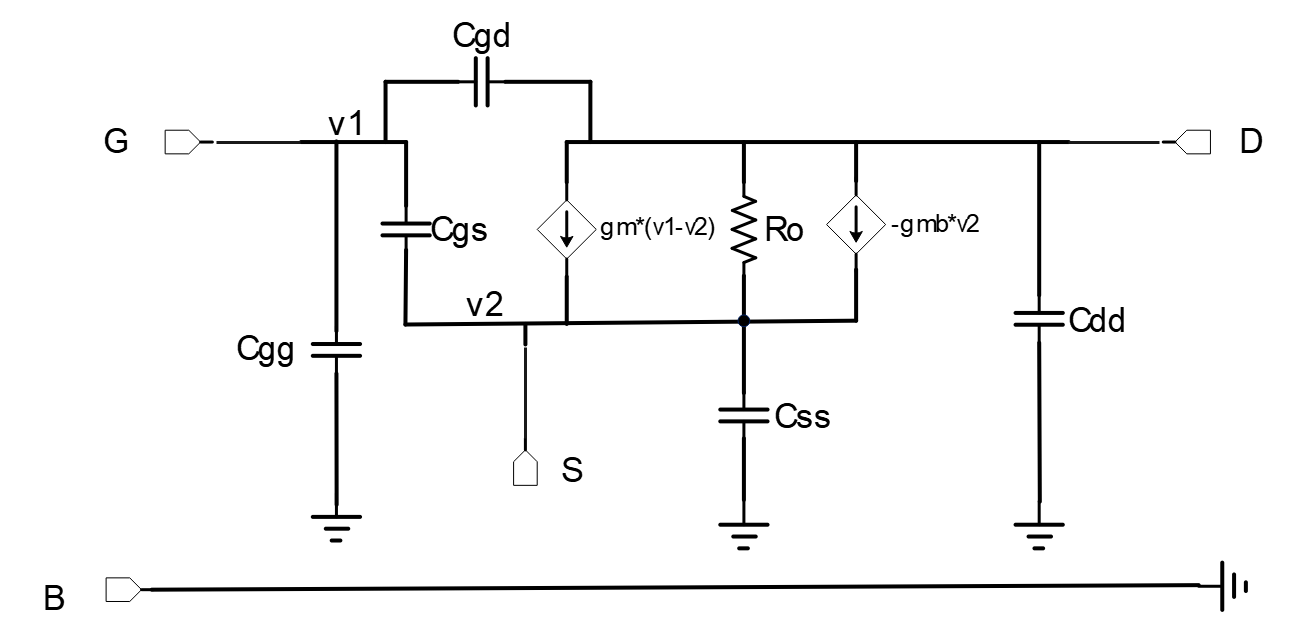
\includegraphics[width=0.7\textwidth]{fig/mos-small-signal-model-2.pdf}
  \caption{CMOS equivalent small-signal model \cite[Figure 2.39]{razavi2002design}, where, Ro is a resistor with resistance $\frac{1}{\text{GDS}}$.}
  \label{fig:mos-small-signal-model-2}
\end{figure}
There are a few points to note:
\begin{enumerate}[partopsep=0pt,topsep=0pt,itemsep=0pt,parsep=0pt]
  \item The role of built-in basic elements ICS and ACVCCS (Appendix \hyperref[appendix:mos-subckt]{B}) is to ensure that ID only functions under DC analysis, while GDS, GM and GMB only function under AC analysis.
  \item The DCAC hybrid analysis or DC analysis computational graph of the equation constructor can execute this circuit module. However, the pure AC analysis computational graph cannot independently run this circuit module: In order to establish the AC analysis equations, it is necessary to first compute [GDS,GM], etc., which are determined by the DC bias voltage. This is different from directly inducing small signal linear equations through TRAN analysis equations (Appendix \hyperref[appendix:TRAN-to-AC-equation]{A}). In fact, Assumption \ref{assumption:intrinsic-params-dependencies} also stipulates that internal variables can depend on the bias voltage signal, but not on the small signals in linear analysis.
  \item The SubModel can freely call external programs, such as using three-dimensional spline interpolation, provided that it ensures compliance with the interface requirements of the corresponding automatic differentiation system.
\end{enumerate}
This submodel-based device model representation method features "equivalent circuit decomposition + dynamic parameters" and shows the following advantages:

\begin{enumerate}[partopsep=0pt,topsep=0pt,itemsep=0pt,parsep=0pt]
  \item Decoupled from circuit network analysis or simulation, the submodel is only responsible for calculating the intrinsic parameters and Jacobian matrix (Section \ref{subsec:subckt-instance-data-structure}). Circuit connectivity is not the submodel's concern.
  \item The syntax and capability boundary of a submodel in calculating intrinsic parameters depend on the compiler's processing of the "SubModel" field in the netlist. This can be implemented easily using various external programs and automatic differential tools.
\end{enumerate}

\subsection{OpAmp Device Sizing: DC Operating Points Optimization Under Different PVT Combinations}
Figure \ref{fig:manually-design} shows the device sizing process in analog circuit design. Specifically, designers connect available devices accessible to the target process into circuits, and adjust the size of each device (such as a CMOS device) based on specific methodologies and experience so that a circuit can fulfill specification requirements under a given area and power consumption constraints. In this process, repeated circuit simulation is done to quantitatively inspect the behavior and performance of a circuit without the need to manufacture the physical circuit.
\begin{figure}[htpb]
  \centering
  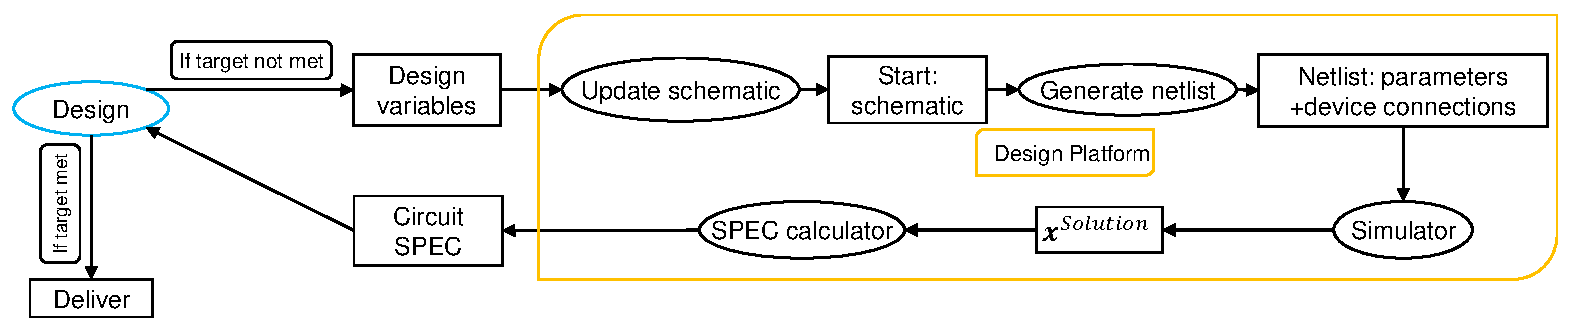
\includegraphics[width=\textwidth]{fig/manually-design.pdf}
  \caption{Manual device sizing: an iterative process}
  \label{fig:manually-design}
\end{figure}

This process can be naturally converted into an optimization problem. The optimization strategy varies depending on whether the gradient is acquirable \cite{zhan2004optimization,agrawal2006circuit,huang2013efficient,nieuwoudt2005multi,peng2016efficient,girardi2011analog,lyu2018batch,wang2014enabling,lyu2017efficient,tang2018parametric}. Take DC simulation as an example. To obtain the gradient, the DC steady-state equations $\bm{F}(\bm{x},\bm{p})=\bm{0}$ naturally provide an implicit mapping from the parameter $\bm{p}$ to the solution $\bm{x}^{solution}$ of the systems of equations, with the Jacobian matrix of this mapping being $\nabla_{\bm{p}}\bm{x}^{solution}=-\nabla_{\bm{x}}\bm{F}\backslash\nabla_{\bm{p}}\bm{F}$, where $\nabla_{\bm{x}}\bm{F},\nabla_{\bm{p}}\bm{F}$ may be directly given by the equations system construction method (computational graph \ref{fig:computational-graph}) described in Section \ref{sec:Joanna}.
With this information, the gradient optimization method (Figure \ref{fig:solve-then-optimize}) can be used.
Note that in an optimization process, the inverse of $\nabla_{\bm{x}}\bm{F}$ does not need to be completely solved.
Instead, it is sufficient to solve a set of linear equations only once during each iteration's gradient backpropagation for a given loss function or constraint function $l$:
$\nabla_{\bm{p}}l(\bm{x}^{solution})=(\nabla_{\bm{p}}\bm{x})^T\cdot\nabla_{\bm{x}}l
=-(\nabla_{\bm{p}}\bm{F})^T\cdot\big(\nabla_{\bm{x}}\bm{F}^T\backslash\nabla_{\bm{x}}l\big)$
\begin{figure}[htpb]
  \centering
    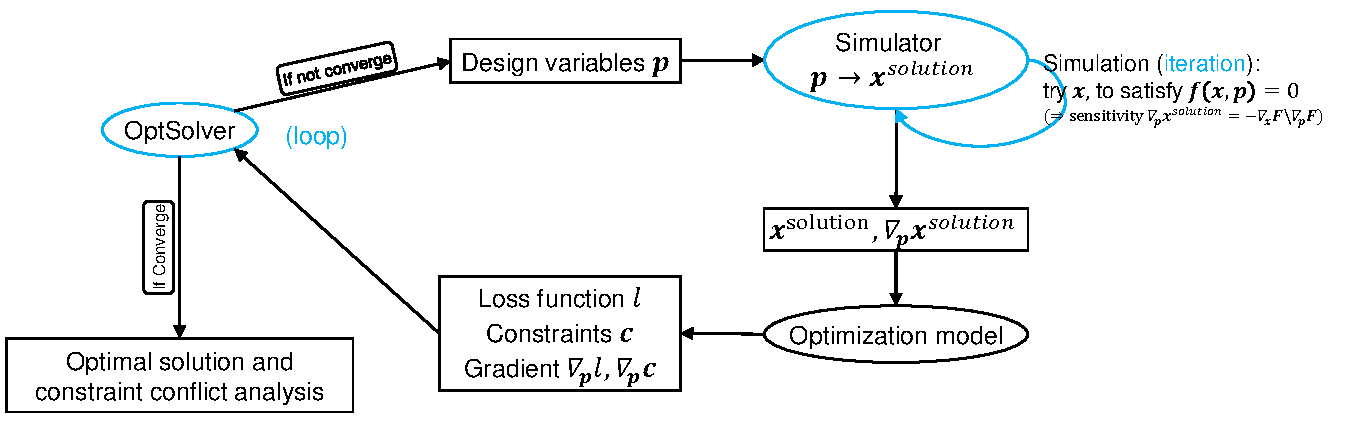
\includegraphics[width = 0.7\textwidth]{fig/solve-then-optimize.pdf}
  \caption{Automatic device sizing}
  \label{fig:solve-then-optimize}
\end{figure}

\begin{figure}[htbp]
  \centering
  \begin{subfigure}{0.3\textwidth}
    \includegraphics[width=\textwidth]{fig/amplifier-diagram.png}
    \caption{OpAmp schematic diagram \cite{OpAmpPNG}}
    \label{subfig:amplifier-diagram}
  \end{subfigure}
  \begin{subfigure}{0.65\textwidth}
    \includegraphics[width=\textwidth]{fig/amplifier-transfer-function.png}
    \caption{Input and output frequency response curves of the OpAmp after sizing}
    \label{subfig:amplifier-transfer-function}
  \end{subfigure}
  \caption{\textbf{(a)}: OpAmp schematic diagram, including the bias circuit and the main circuit, and a total of 17 n-MOSFET and 17 p-MOSFET devices. At the DC operating point, when small-signal disturbance with a given frequency is applied at $V_+,V_-$, an output signal is detected at $V_{out}$. \textbf{(b)}: Frequency response curves of OpAmp after sizing under $Corner=tt,Temperature=27$ conditions, where, va4 and va5 are the two internal nodes in the circuit.}
\end{figure}
Taking an OpAmp (Figure \ref{subfig:amplifier-diagram}) as an example, consider the design variables of the circuit (i.e., the channel length and width of each MOSFET) as the variables to be optimized.
Given the external current and voltage sources Ibias0, Ibias1, and $V_{dd},V_+,V_-$ and the load resistance and capacitance $R_L=200\Omega,C_L=10^{-10}\text{F}$, set the optimization goals as follows:
\begin{enumerate}[partopsep=0pt,topsep=0pt,itemsep=0pt,parsep=0pt]
  \item The DC operating points of all MOSFETs must be saturated under nine PVT conditions defined by $Corner\in[tt,ff,ss],Temperature\in[27,-40,125]$. For example, for an NMOS, its DC bias voltage must satisfy
    \vspace{-1em}
    \[
      \min(V_{gs},V_{ds},V_{sb},V_{gs}-V_{th})\geq0,
      \vspace{-1em}
    \]
    where, $V_{th}$ is subject to MosL,$V_{gs},V_{ds}$. For different PVT conditions, the SubModel needs to load different databases, and therefore the final simulation solutions obtained are also different.
  \item Under the typical condition of $Corner=tt,Temperature=27$, slight fluctuation is allowed for voltage sources $V_+,V_-$ as long as $V_++V_-=5v$ is satisfied. For the DC bias of $V_{out}$, the maximum must be greater than 4.35 V, and the minimum must be less than 0.3 V.
    Because our model (Section \ref{subsec:cmos-model}) is not used in the TRAN analysis, this requirement plays a similar role as the output swing indicator of circuits.
  \item AC analysis is performed on the circuit under the typical condition $Corner=tt$, $Temperature=27$ and a $v_{in+},v_{in-}=\pm0.5$ signal is applied at $V_+,V_-$. The DC gain $gain=20\cdot\log_{10}(|v_{out}|)$ of $V_{out}$ must reach 100.
  \item The design variables of each device meet given symmetry constraints. For example, the input MOSFET pair $M_{n0\_in},M_{n0\_ip}$ have the same size (MosL,MosW), and the current mirrors $M_{p30\_mirr},M_{p20\_mirr},M_{p10\_mirr},M_{p50\_mirr},M_{p60\_mirr}$ have the same channel length (MosL).
\end{enumerate}
\begin{equation}\label{eq:optimization}
  \begin{split}
    \min_{\bm{p}} l &= \max(5-\log_{10}(|\bm{v}[out]|),0)^2 \\
    \st \ \ \ \ \ \ 
    & \forall c\in[tt,ff,ss],t\in[27,-40,125], \\
    & \ \ \ \ \bm{x}_L\preceq\bm{x}^{c,t}\preceq\bm{x}_U;
    Saturation(\bm{x}^{c,t},\bm{p})\succeq\bm{0}; \\
    & \bm{x}^{down}[out]\leq0.3;\bm{x}^{up}[out]\geq4.35; \\
    & \bm{v}=\bm{A}^{tt,27}\backslash\bm{b}^{tt,27}; \ C\cdot\bm{p}=\bm{0}.
  \end{split}
\end{equation}
This design task can be expressed as a constrained optimization problem Prob.\eqref{eq:optimization}. $\bm{p}\to\{\bm{x}^{c,t}\},\bm{x}^{down},\bm{x}^{up}$ is obtained by solving the system of DC equations under corresponding PVT conditions with input bias $V_+,V_-$. And $\bm{v}=\bm{A}^{tt,27}\backslash\bm{b}^{tt,27}\triangleq\bm{A}\ \backslash\bm{b}$ solves the system of AC linear equations under the $Corner=tt$,$temperature=27$ condition, where the matrix elements of $\bm{A}$ are GM, GDS, etc. of each device subject to $\bm{x}^{tt,27},\bm{p}$. We can use a computational graph of mixed DCAC analysis to calculate $\bm{A},\bm{b},\nabla_{\bm{x}}\bm{A},\nabla_{\bm{x}}\bm{b}$ \footnote{$A=i\omega\cdot\nabla_{\bm{x}}\bm{Q}+\nabla_{\bm{x}}\bm{F}$. For a simpler graph implementation, use the DCAC computational graph (instead of $\nabla\bm{Q},\nabla\bm{F}$) to calculate $\nabla A$. This avoids calculating and propagating backward the second derivative of $\bm{Q},\bm{F}$ with regard to $\bm{x}$.}, which can further enable the calculation of $\nabla_{\bm{x}}l,\nabla_{\bm{p}}l$ (Appendix \hyperref[appendix:inv-linear-equation-grad]{C}). $C\cdot\bm{p}=\bm{0}$ represents the direct constraints on design variables, such as a symmetry constraint.

The optimization algorithm is implemented by using the open-source software Ipopt \cite{wachter2006implementation} and includes 72 variables, 27 equality constraints, and 308 inequality constraints to be solved. It took 356 seconds to run the whole process (including compiling Julia code and parsing netlist, etc.) on six threads on Intel(R) Core(TM) i7-8700 CPU at 3.20 GHz. Figure \ref{subfig:amplifier-transfer-function} shows the frequency response curve of the optimized circuit. The experimental results show that:
\begin{enumerate}[partopsep=0pt,topsep=0pt,itemsep=0pt,parsep=0pt]
  \item In hierarchical circuit simulation or sizing based on the computational graph, the device model and solution algorithm are decoupled from each other, allowing for high flexibility and efficiency.
  \item The parameters in the computational graph are processed to function as variables, making gradient optimization of many indicators simpler and easier.
\end{enumerate}
Note that the preceding experiments only consider the operation points of devices and circuit DC gains under typical conditions. To complete the design, more indicators (even discrete value indicators) need to be introduced into the optimization problem. There is no shortcut to properly integrating all indicators into the optimization framework, which however will not be addressed here.






\section{Conclusion}
In this paper, the static parameters of the circuit are processed as runtime variables in simulation, and the structural information and behavioral information of the circuit module/device are decoupled as "equivalent subcircuit decomposition + submodel-computed dynamic parameters". These further derive the computational graph representation of the equations system constructor for hierarchical circuits with circuit modules as the compute units of the computational graph. According to the two simple examples, this approach facilitates the decoupling and flexible interaction between netlists, models, and simulation and optimization algorithms. However, some problems exist with this approach. For example, because the variable gradient will be passed across the layers of a circuit, the topology analysis for circuit equations solvability and DAE-Index no longer works, requiring a more general hierarchical analysis theory. In the future, this approach will gain better generalization by supporting BSIM and more simulation types with more effects (i.e., S parameter or thermal effect) considered. Faster simulation is also possible if the program itself is optimized and the support for fast-SPICE technology is added.

\section*{Acknowledgment}
\addcontentsline{toc}{section}{Acknowledgment}
I would like to thank my colleagues at Turing Department. It's been both a pleasure and an honor to work with them. This work has been also supported by many EDA and HDL experts, including Waisum Wang, Jiewen Fan, Zuochang Ye, Yang Lu, Shangxia Fang, Guoyong Shi, and Yu Ji. Special thanks go to Zhenya Zhou, Jiawei Zhuang, Long Wang, and Yuwei Fan for their kind help.

\addcontentsline{toc}{section}{References}
\bibliography{ref}
\section*{Appendix}
\addcontentsline{toc}{section}{Appendix}
\renewcommand\thesubsection{\Alph{subsection}}
\subsection{TRAN Analysis Induced AC Analysis Equation}\label{appendix:TRAN-to-AC-equation}
To solve the transient equation \ref{eq:flat-equation} and the DC steady-state equation $\bm{F}(\bm{x}, \bm{p})=\bm{0}$,
the Newton-Raphson method calculates $\bm{Q},\bm{F}\in\mr^N$ and the Jacobian matrix $\nabla_{\bm{x}}\bm{Q},\nabla_{\bm{x}}\bm{F}\in\mr^{N\times N}$ repeatedly.
In AC small-signal analysis, consider applying perturbation $\delta\bm{x},\delta\bm{p}$ around the steady-state solution $\bm{x},\bm{p}$ and linearizing \ref{eq:flat-equation} as follows:

\[
\nabla_{\bm{x}}\bm{Q}\cdot\dot{\delta}\bm{x}
+\nabla_{\bm{p}}\bm{Q}\cdot\dot{\delta}\bm{p}
+\nabla_{\bm{x}}\bm{F}\cdot\delta\bm{x}
+\nabla_{\bm{p}}\bm{F}\cdot\delta\bm{p}=\bm{0}
\]
Let $\delta\bm{x},\delta\bm{p}$ be a small signal with an angular frequency of $\omega$: 
$\delta\bm{x}=\bm{\epsilon}_{\bm{x}}\cdot e^{i\omega t},\delta\bm{p}=\bm{\epsilon}_{\bm{p}}\cdot e^{i\omega t}$.
Then the system of linear equations of AC small-signal analysis is
\begin{equation}\label{eq:flat-ac-equation}
(i\omega\cdot\nabla_{\bm{x}}\bm{Q}+\nabla_{\bm{x}}\bm{F})\cdot\bm{\epsilon}_{\bm{x}}
= (i\omega\cdot\nabla_{\bm{p}}\bm{Q}+\nabla_{\bm{p}}\bm{F})\cdot\bm{\epsilon}_{\bm{p}}
\end{equation}

\subsection{CMOS Subcircuit}\label{appendix:mos-subckt}
\begin{lstlisting}[language=json,numbers=none,
caption={CMOS subcircuit},label=lst:mos-subckt]
"NMOSTYPE":{
  "ExternalNodes":["gate","source","drain","bulk"],
  "InputParams":["MosL","MosW"],
  "InternalNodes":[],
  "SubModel":{
    "Analysis":["DC","TRAN"],
    "ModelLoader":"SimInfo->lut.MosLookup(\"NMOSTYPE\",
      /path/to/data; SimInfo=SimInfo)",
    "IntrinsicParams":
      ["ID","GDS","CDD","CSS","CGG","CGS","CGD","GM","GMB"]
  },
  "Schematic":{
    "ids":{
      "MasterName":"ICS",
      "ExternalNodes":{"input":"source","output":"drain"},
      "InputParams":{"dc":"ID","ac":0}
    },
    "template":{
      "MasterName":"MosSmallSignalTemplate",
      "ExternalNodes":{
        "gate":"gate","source":"source",
        "drain":"drain","bulk":"bulk"
      },
      "InputParams":{
        "GDS":"GDS","CDD":"CDD","CSS":"CSS","CGG":"CGG",
        "CGS":"CGS","CGD":"CGD","GM":"GM","GMB":"GMB"
      }
    }
  }
}
\end{lstlisting}
\begin{lstlisting}[language=json,numbers=none,
caption={MosSmallSignalTemplate: Small signal equivalent circuit decomposition},label=lst:mos-small-signal-subckt]
"MosSmallSignalTemplate":{
  "ExternalNodes":["gate","source","drain","bulk"],
  "InputParams":["GDS","CDD","CSS","CGG","CGS","CGD","GM","GMB"],
  "InternalNodes":[],
  "Schematic":{
    "infr":{
      "MasterName":"resistor",
      "ExternalNodes":{"left":"drain","right":"source"},
      "InputParams":{"resistance":1e1000}
    },
    "gds":{
      "MasterName":"ACVCCS",
      "ExternalNodes":{"left":"drain","right":"source","input":"drain","output":"source"},
      "InputParams":{"MF":"GDS"}
    },
    "cdd":{
      "MasterName":"capacitor",
      "ExternalNodes":{"input":"drain","output":"bulk"},
      "InputParams":{"capacitance":"CDD"}
    },
    "css":{
      "MasterName":"capacitor",
      "ExternalNodes":{"input":"source","output":"bulk"},
      "InputParams":{"capacitance":"CSS"}
    },
    "cgg":{
      "MasterName":"capacitor",
      "ExternalNodes":{"input":"gate","output":"bulk"},
      "InputParams":{"capacitance":"CGG"}
    },
    "cgs":{
      "MasterName":"capacitor",
      "ExternalNodes":{"input":"gate","output":"source"},
      "InputParams":{"capacitance":"CGS"}
    },
    "cgd":{
      "MasterName":"capacitor",
      "ExternalNodes":{"input":"gate","output":"drain"},
      "InputParams":{"capacitance":"CGD"}
    },
    "gm":{
      "MasterName":"ACVCCS",
      "ExternalNodes":{
        "left":"gate","right":"source","input":"drain","output":"source"
      },
      "InputParams":{"MF":"GM"}
    },
    "gmb":{
      "MasterName":"ACVCCS",
      "ExternalNodes":{
        "left":"bulk","right":"source","input":"drain","output":"source"
      },
      "InputParams":{"MF":"GMB"}
    }
  }
}
\end{lstlisting}

\subsection{Gradient Backpropagation of the Solution of a Linear Equations System}\label{appendix:inv-linear-equation-grad}
Consider a system of real linear equations $\bm{A}(\bm{x})\bm{v}=\bm{b}(\bm{x})$ with respect to $\bm{v}$,
where $\bm{A},\bm{b}$ are nonlinearly dependent on $\bm{x}$ being a sparse matrix/vector, and
$\nabla_{\bm{x}}\bm{A},\nabla_{\bm{x}}\bm{b}$
are computable, then $\bm{v}$ will also be nonlinearly dependent on $\bm{x}$. Differentiating the system of equations yields:
\[
(\bm{A}+\nabla_{\bm{x}}\bm{A}\cdot\ud\bm{x})\cdot
(\bm{v}+\nabla_{\bm{x}}\bm{v}\cdot\ud\bm{x})
=\bm{b}+\nabla_{\bm{x}}\bm{b}\cdot\ud\bm{x}
\]
When the zeroth and second order terms are dropped, the following equation holds for any $\ud\bm{x}$
\begin{equation}\label{eq:inv-full-differentiation}
\nabla_{\bm{x}}\bm{A}\cdot\ud\bm{x}\cdot\bm{v}
+\bm{A}\cdot\nabla_{\bm{x}}\bm{v}\cdot\ud\bm{x}
=\nabla_{\bm{x}}\bm{b}\cdot\ud\bm{x},
\end{equation}
Assume a loss function $l(\bm{v})$, whose gradient $\nabla_{\bm{v}}l$ can be calculated.
Backpropagating the gradient to $\bm{x}$ is equivalent to finding the solution of
$\nabla_{\bm{x}}l=\nabla_{\bm{v}}l\cdot\nabla_{\bm{x}}\bm{v}$.
In fact, we do not need to actually calculate $\nabla_{\bm{x}}\bm{v}$ and store the data, which can be rather dense.
According to Equation \ref{eq:inv-full-differentiation}, we have
\[
\begin{split}
& \nabla_{\bm{x}}\bm{v}\cdot\ud\bm{x}
= \bm{A}^{-1}\cdot\big(\nabla_{\bm{x}}\bm{b}\cdot\ud\bm{x}-
\nabla_{\bm{x}}\bm{A}\cdot\ud\bm{x}\cdot\bm{v}\big),\forall \ud\bm{x}, \\
\Rightarrow
& \nabla_{\bm{v}}l\cdot\nabla_{\bm{x}}\bm{v}\cdot\ud\bm{x}
= (\nabla_{\bm{v}}l\cdot\bm{A}^{-1})\cdot\big(\nabla_{\bm{x}}\bm{b}\cdot\ud\bm{x}-
\nabla_{\bm{x}}\bm{A}\cdot\ud\bm{x}\cdot\bm{v}\big),\forall \ud\bm{x}, \\
\end{split}
\]
Therefore, in order to calculate $\nabla_{\bm{v}}l\cdot\nabla_{\bm{x}}\bm{v}$,
we only need to solve the sparse matrix linear equations system $\nabla_{\bm{v}}l\cdot\bm{A}^{-1}$ once in advance,
element-wisely set the values of $\ud\bm{x}$ to 1 and the rest to 0. Then, we obtain
$\nabla_{\bm{x}}l=\nabla_{\bm{v}}l\cdot\nabla_{\bm{x}}\bm{v}$.

For the case of a set of complex linear equations, a similar discussion can also be carried out using the Wirtinger derivative.

\end{document}



